\documentclass[a4paper]{report}   

\usepackage[utf8]{inputenc}
\usepackage[francais]{babel}
\usepackage{graphicx}
\usepackage{algorithmic}
\usepackage{amsmath}

\renewcommand{\thesection}{\Roman{section}}
\usepackage[]{algorithm2e}

\title{Détection d'anomalies de classification dans l'IoT via Machine Learning}
\author{Antoine Urban, Yohan Chalier}
\date{\today}

\begin{document}

\begin{titlepage}
	\centering
	\vspace{1cm}
	{\scshape\LARGE Télécom ParisTech \par}
	\vspace{1cm}
	{\scshape\Large Projet de filière SR2I \par}
	\vspace{1.5cm}
	{\huge\bfseries Détection d'anomalies de classification dans l'IoT via Machine Learning\par}
	\vspace{2cm}
	{\Large\itshape Antoine Urban, Yohan Chalier \par}
	\vfill
	encadré par\par
	Jean-Philippe \textsc{Monteuuis}\par
	Houda \textsc{Labiod}
	\vfill

% Bottom of the page
	{\large \today\par}
\end{titlepage}



\begin{abstract}
Dans le contexte de l’internet des objets, les messages peuvent contenir de fausses informations générées par un utilisateur authentifié. Par conséquence, les mécanismes de sécurité reposant sur le chiffrement et la signature sont inutiles face à ces attaques. Les algorithmes reposant sur l’apprentissage machine (Machine Learning) permet de classer si un objet  émettant des données est malicieux ou non 
\end{abstract}

\section{Introduction}
L’exercice de la conduite est synonyme de changements constant. Ainsi, lorsque nous conduisons, notre attention est tout entière consacré à notre environnement, car notre sécurité est celle des personnes qui nous entourent sont en jeu. Nous prêtons ainsi naturellement une attention toute particulière aux obstacles qui peuvent surgir, qu’il s’agisse tout simplement d’autres voitures partageant la route, des piétons ou encore des motocyclistes. 
Longtemps objets fantasmés, les véhicules autonomes deviennent aujourd’hui réalités grâce aux incroyables progrès réalisés dans les domaines de l’intelligence artificielle et du développement de capteurs. Si ces processus visent à remplacer le conducteur humain, il semble naturel qu’ils prêtent la même attention aux obstacles. Les méthodes utilisées se doivent d’être fiables et performante, car en matière de sécurité, le droit à l’erreur n’existe pas ! \\

Dans ce travail, nous nous concentrerons sur les 3 types d’obstacles les plus communs sur une route:
\begin{itemize}
\item Une voiture ;
\item Une moto;
\item Un piéton.

\end{itemize}

Tout travail sur l’analyse d’obstacles nécessite la détection préalable de régions d’intérêt en utilisant par exemple la méthode du “point-in-polygon”\cite{ref1}, ou encore à l’aide de capteurs à ultrasons et d’analyse de signal\cite{ref2}. Ce travail n’a pas comme objectif de revenir sur l’utilisation de ces techniques, mais se concentrera sur l’analyse à posteriori des dimensions ainsi collectées avec pour but de proposer une classification efficace. 

\subsection*{Objectifs}
A travers un cas simple, nous cherchons à vérifier l’appartenance d’un objet à une classe (e.g. un véhicule) en utilisant un algorithme de machine learning et les dimensions de l’objet. Il s’agit donc de proposer un modèle de classification multi-classes en réalisant un classeur à partir d’un algorithme d’apprentissage supervisé. 
Au préalable, nous nous assurons de trouver des bases de données avec les dimensions pour chacune des classes pour entraîner et valider notre modèle. 
Ensuite, nous proposerons une méthodologie de sélection d’un algorithme d’apprentissage supervisé en évaluant leur précision et leur efficacité respectives. Dans ce travail, nous avons considérés les algorithmes (c) suivant: 
\begin{itemize}
\item Réseau de Neurones (c = 1) ;
\item Adaboost (c = 2);
\item SVM(c=3);
\item Random Forest (c=4).
\end{itemize}
\medbreak

La fonction suivante permet de résumer le déroulé du processus de prédiction:\\
\RestyleAlgo{boxruled}

\begin{algorithm}[H]
\SetAlgoLined
\textbf{Donnée:} Un message i envoyé par un objet communicant contenant:\\
\begin{itemize}
	\item Classe de l'objet(Classe_{i}= (Voiture, moto, piéton))
	
	\item Dimension de l’objet (Longueur: L_{i}; Largeur: l_{i}).
	
\end{itemize}

\bigbreak

\KwResult{Détection des objets malicieux}
\medbreak
\eIf{function (Class, Longueur, Largeur)}{
  Return “malicieux”\;
  }{
  Return “non malicieux”\;
}
\caption{Fonction de production}
\end{algorithm}
\medbreak


\begin{center}
   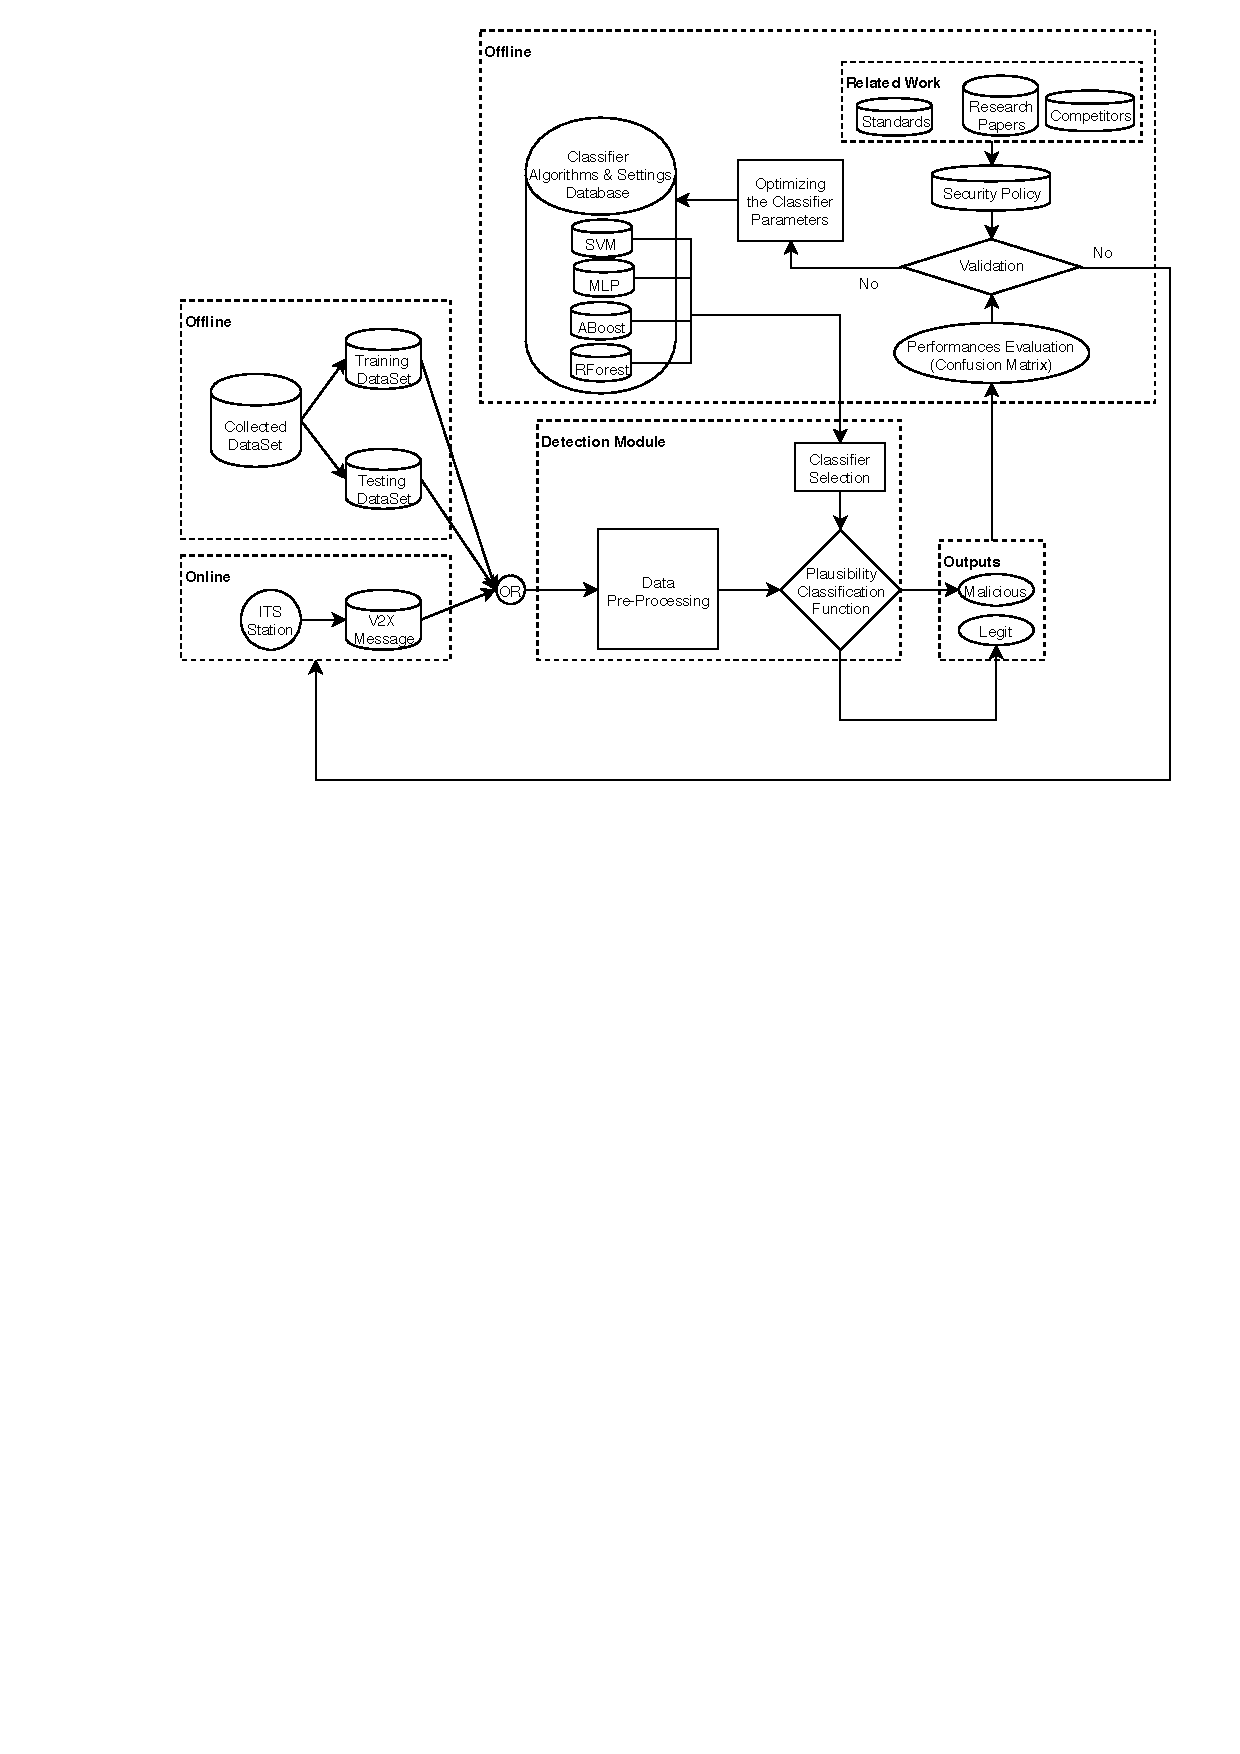
\includegraphics[width=\textwidth]{MLFramework.pdf}
\end{center}



\section{Méthode d'évaluation}


\subsection{Matrice de confusion}
Une technique pour évaluer la performance d’un algorithme de classification est d’utiliser une matrice de confusion. Il s’agit d’un résumé des résultats de prédiction sur un problème de classification, qui donne un aperçu du degré de confusion de notre modèle. 

\subsubsection{Terminologie}
Pour définir de manière formelle une matrice de confusion, il convient d’introduire les termes suivant: 
\begin{itemize}
\item TP (Vrai Positif): item correctement détecté positif 
\item FP (Faux Positif): item déclaré positif, là où il est en réalité négatif.
\item FN (Faux négatif): item déclaré négatif alors qu'il était en réalité positif.
\item TN (Vrai négatif): item correctement détecté comme négatif
\end{itemize}
\\

Ces derniers permettent de définir la classification, correct ou non, des objets données en entrée de notre fonction. Nous pouvons dès lors construire la matrice suivante: 

\begin{tabular}{l|l|c|c|cc}
\multicolumn{2}{c}{}&\multicolumn{2}{c}{Actual class}&\\
\cline{3-4}
\multicolumn{2}{c|}{}&Positive&Negative&\multicolumn{1}{c}{}\\
\cline{2-4}
\multirow{Predicted classes}& Positive & $TP$ & $FP$ & $PPV$ & \multicolumn{1}{c}{$FDR$}\\
\cline{2-4}
& Negative & $FN$ & $TN$ & $FOR$& \multicolumn{1}{c}{$NPV$} \\
\cline{2-4}
\multicolumn{1}{c}{} & \multicolumn{1}{c}{}
& \multicolumn{1}{c}{$TPR$} & \multicolumn{    1}{c}{$FPR$} & \multicolumn{1}{c}{}\\
\hhline{~~~~~~}
\multicolumn{2}{c}{} 
& \multicolumn{1}{c}{$FNR$} & \multicolumn{1}{c}{$TNR$} & \multicolumn{1}{c}{}\\
\end{tabular}
\bigbreak

Pour la suite, et pour comprendre cette matrice, il convient d'introduire les résulats suivants:\\
\begin{itemize}\setlength{\itemsep}{5mm}
	\item Ratio de Vrai positif: TPR=\dfrac{TP}{TP+FN}
	
	\item Ratio de Vrai négatif: TNR=\dfrac{TN}{TN+FP}
	
	\item Ratio de Vrai positif: TPR=\dfrac{TP}{TP+FN}
	
	\item Ratio de Vrai négatif: TNR=\dfrac{TN}{TN+FP}
	
	\item Ratio de Faux positif: FPR=\dfrac{FP}{TP+TN}
	
	\item Ratio de Faux négatif: FNR=\dfrac{FN}{TP+FN}
	
	\item Valeur prédictive positive: PPV=\dfrac{TP}{TP+FP}
	
	\item Valeur prédictive négative: NPV=\dfrac{TN}{TN+FN}
	
	\item Taux de fausses découvertes: TPR=\dfrac{FP}{TP+FP}
	
	\item Taux de fausses omissions: FOR=\dfrac{FN}{TN+FN}
	
\end{itemize}
\bigskip\bigskip

Ce mode de représentation permet non seulement de mettre en évidence les erreurs qui sont faites par votre classificateur, mais surtout des types d'erreurs qui sont commises. En effet, l’utilisation de la seule précision peut être trompeuse dans la mesure où le nombre d’observation dans chaque classe est inégale. 
Pour illustrer ce phénomène, prenons un exemple précis. Considérons l’algorithme SVM (support vector Machine) avec les paramètres suivants:
\medbreak

\fbox{\begin{minipage}[t]{\textwidth}\begin{small}
C=0.1, cache--size=200, class--weight=None, coef0=0.0, decision--function--shape='ovr', degree=3, gamma='auto', kernel='linear', max--iter=-1, probability=False, randomState=None, shrinking=True,  tol=1e-05, verbose=False
\end{small}\end{minipage}}
\medbreak

La précisions de cet algorithme avec ces paramètres est égale à 0.96660 et renvoie la matrice de confusion suivante:

\medskip
\begin{center}
\begin{bmatrix}
 2771&74 \\ 
 239&  239
\end{bmatrix}
\end{center}

\medskip
Nous remarquons bien que la classification est loin d’être satisfaisante alors que le score de précision est, lui, important. Il y a en effet dans ce dernier aucune pondération. Si une classe contenant un nombre de paramètres important est bien classifiée, elle peut “masquer” les mauvais résultats obtenus pour d’autres classes plus petites.

\subsubsection{Score F1}


\begin{thebibliography}{9}
\bibitem{ref1}
          Deepika, N AND Sajith Variyar, V. V.,
          Obstacle classification and detection for vision based navigation for autonomous driving,
          Addison Wesley, Massachusetts,
          IEEEl,
          2017.
     
         
\bibitem{red2}
          Gerard Gibbs and Huamin Jia and Irfan Madani,
          Obstacle Detection with Ultrasonic Sensors and Signal Analysis Metrics,
          Transportation Research Procedia,
          2017.
          
\end{thebibliography}



\end{document}